\documentclass[12pt,twoside]{article}
\usepackage[dvipsnames]{xcolor}
\usepackage{tikz,graphicx,amsmath,amsfonts,amscd,amssymb,bm,cite,epsfig,epsf,url}
\usepackage[hang,flushmargin]{footmisc}
\usepackage[colorlinks=true,urlcolor=blue,citecolor=blue]{hyperref}
\usepackage{amsthm,multirow,wasysym,appendix}
\usepackage{array,subcaption} 
% \usepackage[small,bf]{caption}
\usepackage{bbm}
\usepackage{pgfplots}
\usetikzlibrary{spy}
\usepgfplotslibrary{external}
\usepgfplotslibrary{fillbetween}
\usetikzlibrary{arrows,automata}
\usepackage{thmtools}
\usepackage{blkarray} 
\usepackage{textcomp}
\usepackage[left=0.8in,right=1.0in,top=1.0in,bottom=1.0in]{geometry}


\title{1001 Data Analysis Project 3 Report - gjd9961}

\begin{document}

\maketitle

\section*{Introduction}

The purpose of this report is to explain the results obtained from the statistical analysis of the "Movie Ratings Data-Set". The methods used in this analysis include but are not limited to: PCA, KMeans, K-Nearest-Neighbors, and Nueral Networks.  

\section*{Question 1: Personality Factors and PCA}

Before beginnings the first part of my analysis, I decided to fill in missing values in the dataframe provided by using the mean of each column. After the data-set was mean filled, I applied PCA, and inspected the eigenvectors and eigenvalues of the resulting covariance matrix. Looking at the eigenvalues, the first 10 principle components explained roughly 55\% of the variance of the dataset. The remaining principle components had eigenvalues less than or equal to 1. For the sake of interpritability and simplicity, I did not use the Kaiser Rule, and rather disregarded these less meaningful principle components, and only used the top 10.

\begin{figure}[h!]
    \centering
    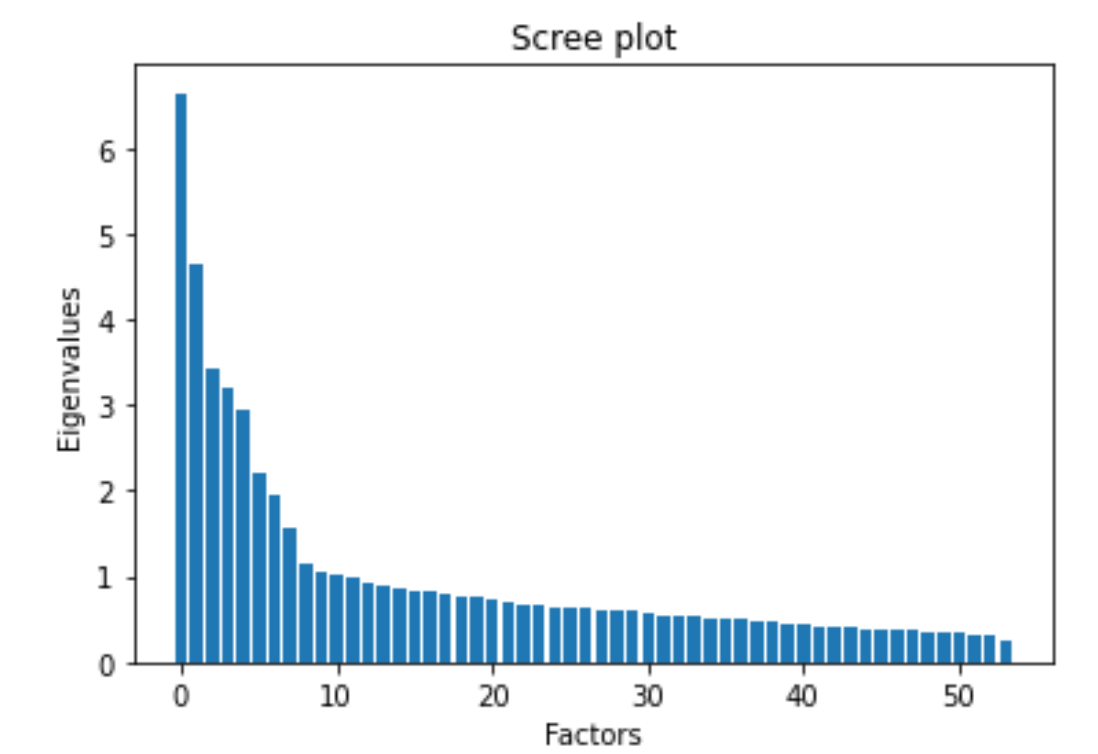
\includegraphics[scale=.9]{scree plot.png}
    \caption{Scree Plot of Eigenvalues}
    \label{fig:my_label}
\end{figure}

In my python Notebook, I analyzed the loading matrix to identify which individual factors comprised each principle component by inspecting the loadings matrix. I then semantically interpreted the ten most meaningful principle components in the following way:\\

\textbf{10 Most Meaningful Principle Components, Semantic Interpretation:}
\begin{enumerate}
    \item Enthusiastic vs negative mentality
    \item Anxious/Impressioanble/Empathetic vs Not
    \item Shy vs Assertive
    \item Avoidant vs Confrontational
    \item structured v unstructured personality
    \item Type A vs Type B Personality
    \item Casual Watcher vs Immersed in the Movie
    \item Attentive and interested or disinterested and distracted
    \item Artistic vs non Artistic
\item- Artistic vs Inventive
\end{enumerate}

A more detailed breakdown of the individual components of the PCs is available in the code.

\section*{Question 2: Plot the PCs}
As there were 10 principle components, and therefore 45 combinations of 2 PCs with 45 plots, I will omit the plots from this report. If you wish to see them, check out the code in the zip file.

\section*{Question 3: Identify Clusters in the New Space}
Initially during my attempt to cluster individuals in the movie rating data-set, I tried finding clusters in pairwise comparisons between principle components. Essentially, I was looking at the plots derived in part 2, and trying to run KMeans clustering algorithm on these plots, and finding that in almost every pairwise comparison, the optimal clusters was 2 clusters. This was not very informative, as the minimum amount of clusters by definition of the KMeans algorithm is 2. So clearly something wasn't working.

I then tried clustering the users in the data-set by using their personality questions data in the PCA-altered form. This was much more informative, and as I ran KMeans in this higher dimensional space, I found that the optimal amount of clusters was approximately 12 (much more meaningful than 2). I used the silhouette method, to achieve the ideal number of clusters. The plots in Figure 2 illustrates how the KMeans sum of errors changed as the number of clusters varied.  

\begin{figure}[h!]
    \centering
    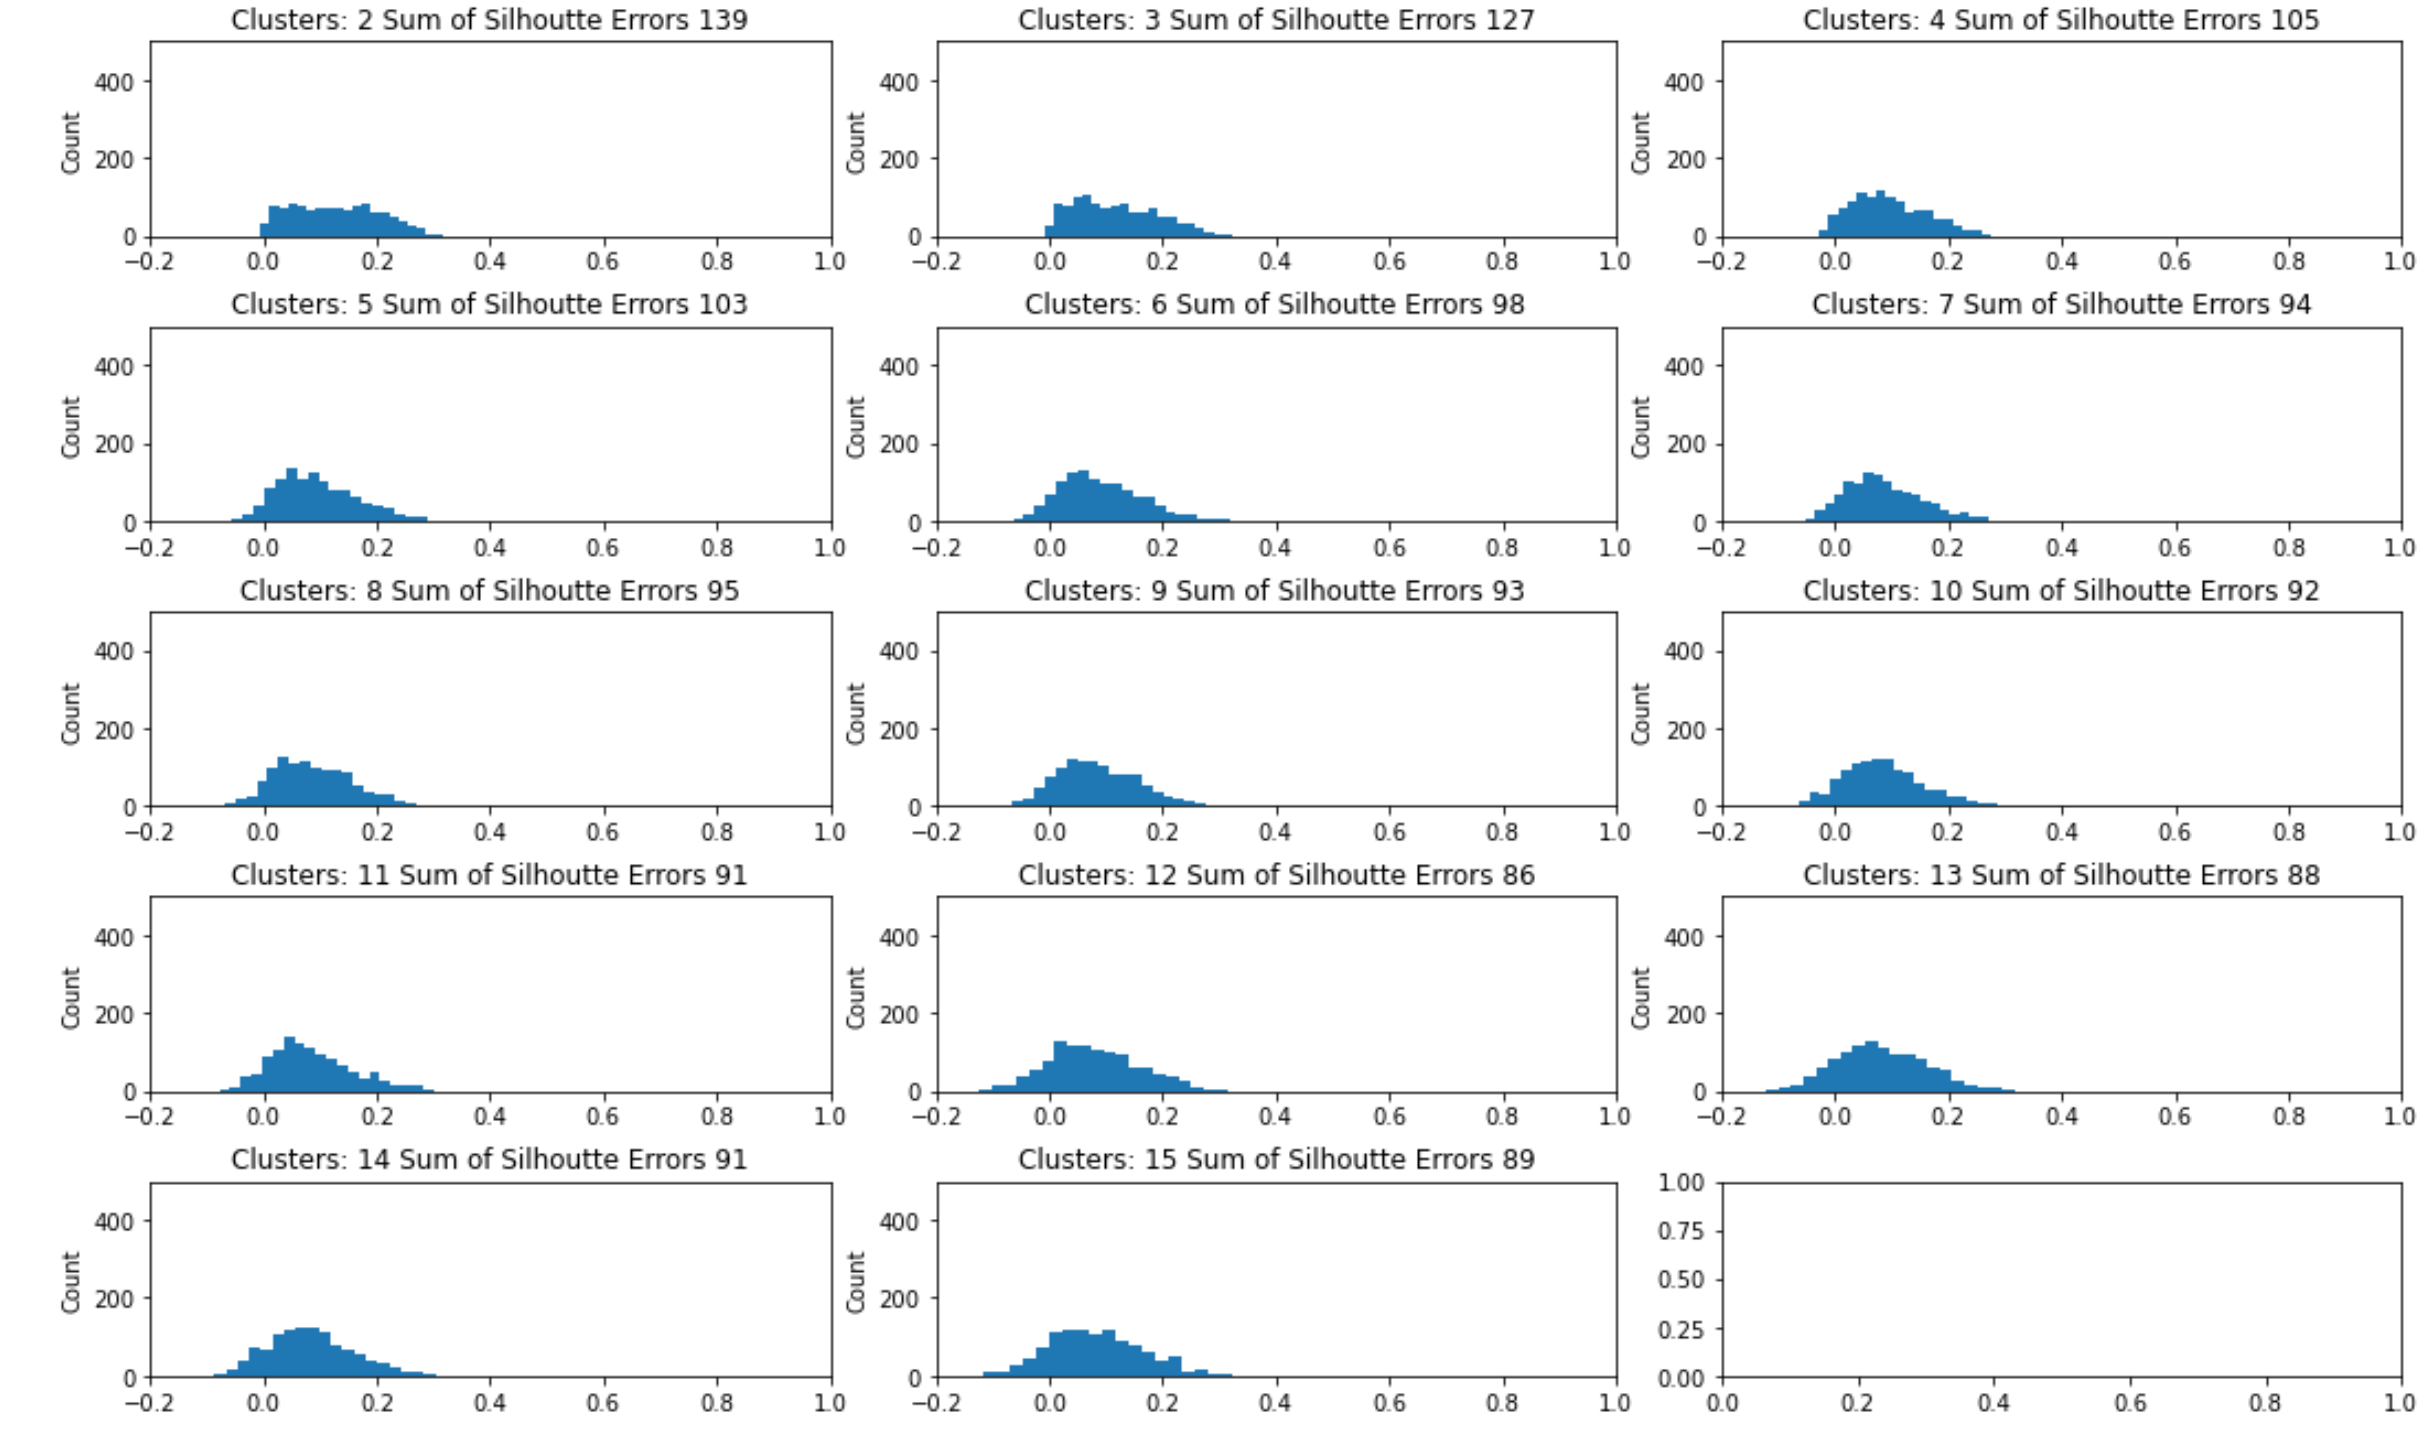
\includegraphics[scale=.7]{kmeans plots.png}
    \caption{Plot of Kmeans Sum of Errors by Number of Clusters}
    \label{fig:my_label}
\end{figure}


\section*{Question 4: Use PCA Clusters to Perform Classification}
Using the clusters I identified in Question 3, I implemented the KNearestNeighbors scitkit-learn algorithm to predict movie scores based on personality traits identified through PCA. I used KFolds cross-validation to split my dataset into 10 different train/test splits. For each of these train/test splits, I tried varying inputs of how many neighbors the KNearestNeighbors function should use when classifying. I did so to try to maximize the AUC score. 

What I found is that beyond using 20-25 neighbors to classify which cluster a user belonged to based on movie ratings, there were diminishing returns associated with the AUC, with the average AUC score of each train/test split for each number of neighbors maxed out around 95-97\%. 

\begin{figure}[h!]
    \centering
    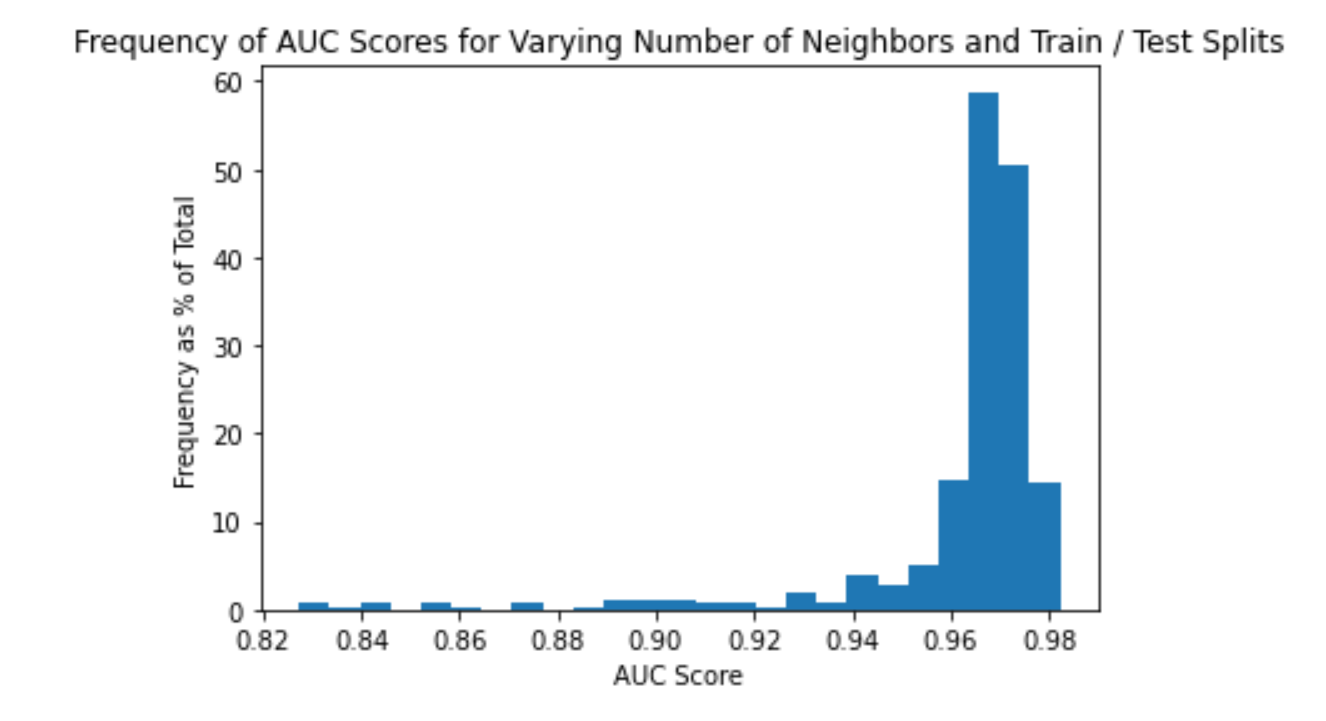
\includegraphics[scale=.9]{auc scores.png}
    \caption{Average AUC Scores For Varying # Of Neighbors and Train / Test Splits}
    \label{fig:my_label}
\end{figure}


\section*{Question 5: Neural Network Prediction of Movie Ratings}
I chose to use a simple Neural Network model from Sci-Kit Learn called MLP CLassifier. The model would use all but 1 column, to predict the excluded column in the dataset. In other words, the model would include all possible data points, (personality questions, movie scores, etc.) to predict any given column of movie ratings. 

I used a simple train/test split, with a 70/30 train testing ratio. I printed the confusion matrix and classification report to evaluate the results for predicting the movie ratings of the movie "Anaconda (1997)". On 330 observations worth of training data, the model performed relatively well, with an weighted average precision of 80\%, recall of 85\%, and f-1 score of .82. However, this is a bit misleading as many of the values in the train and test splits were ratings of value "2" which was the rounded down mean-filled value. Thus, the model had exceptional recall and precision for movie ratings of "2", but very poor recall for ratings of other values. In other words, the model had learned that it was very efficient to simply guess the most common rating.

\begin{figure}[h!]
    \centering
    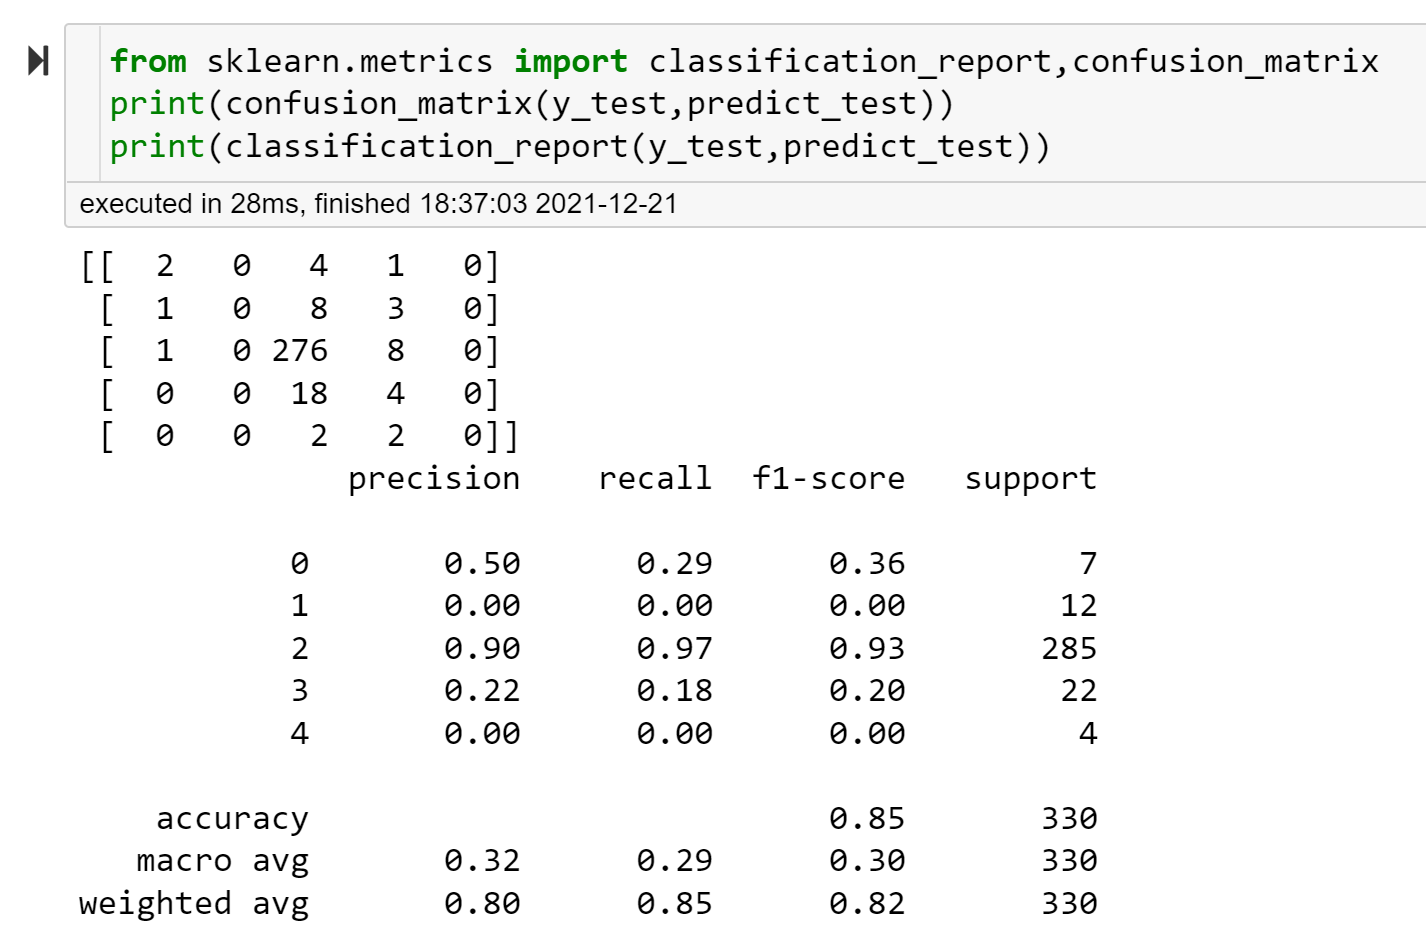
\includegraphics[scale=.9]{ml precision.png}
    \caption{Confusion Matrix and Classifiation Report of "Anaconda (1997")}
    \label{fig:my_label}
\end{figure}


\end{document}